\section{Problem Definition}
In this assignment, it is asked to individually gather info about pilot production sample and future batch production (100 pieces).
Also, sample production in real-life conditions is required to be simulated and organized.
This report is a result of this assignment, which conducted the analysis on the \textbf{prototype of a new seat for economy class cabin}
designed by the author. The following sections will be included in this report:
\begin{itemize}
    \item Construction of the seat (Section \ref{sec:Constr})
    \item BOM analysis (Section \ref{sec:BOM}, also the part type definition is also given in this section)
    \item Technical conditions for production (Section \ref{sec:TechCon})
    \item Production process description (Section \ref{sec:ProdProc})
    \item The staff required for production (Section \ref{sec:Staff})
\end{itemize}

The seat for the economy-class cabin is a common part of the aircraft cabin, and it is also a part that is easy to be produced.
Typically, the seat for economy class should be light, comfortable, and easy to be repaired or refurbished.
Based on this requirement, the author designed a seat for the economy-class cabin, which is shown in Figure \ref{fig:Seat}.

\begin{figure}[!htp]
    \centering
    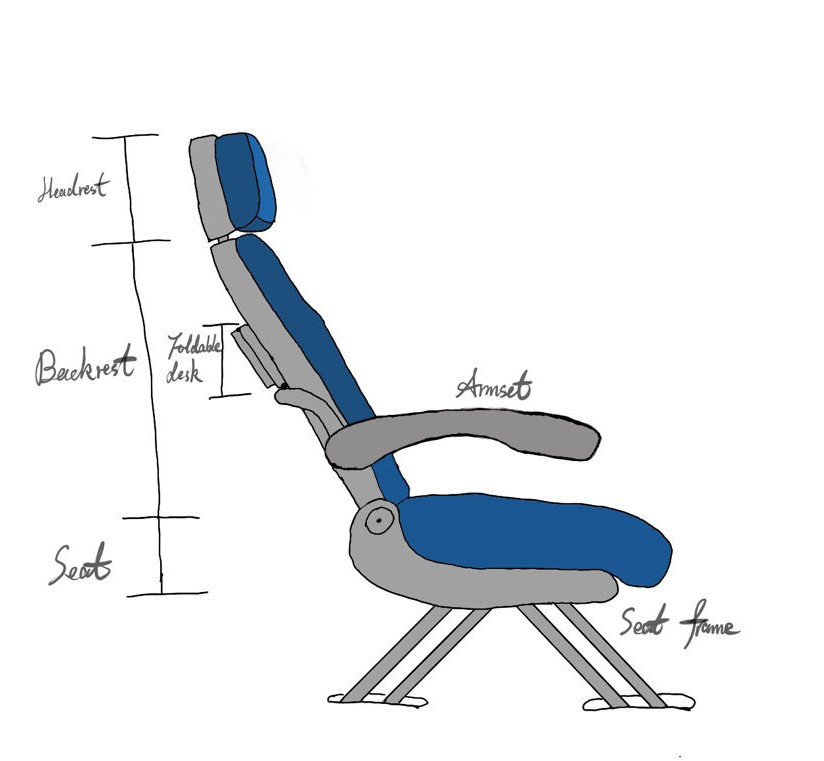
\includegraphics[width=0.9\textwidth]{images/Seat.jpg}
    \caption{The prototype of the seat for economy class cabin (the support legs are not shown completely in the figure)}
    \label{fig:Seat}
\end{figure}

The seat is designed to provide passengers with a comfortable and enjoyable flying experience while being lightweight, durable, and easy to maintain. The dimensions of the seat have been optimized for passenger comfort and space efficiency, with a width of 17 inches (43.18 cm) to accommodate most passengers and a pitch of 31 inches (78.74 cm) to provide ample legroom.

The frame of the seat is made of lightweight composite materials or plastics that are strong and durable, yet light enough to reduce weight and fuel consumption. The cushion covers of the seat are made of high-quality polyurethane foam that provides excellent support and comfort for passengers during long flights.

To enhance passenger comfort, the seat features a polyurethane-filled headrest for optimal neck support and comfort. Armrests provide additional support and can be adjusted to suit passengers of different sizes. 

The seat is designed with a recline function that allows passengers to adjust the angle of the seat for increased relaxation and comfort. The design also allows for quick and easy maintenance, repair, and refurbishment to minimize downtime and costs
by using modular components that can be easily replaced or repaired. For example, the cushions and covers are pre-assembled and can be easily applied to the seat with specially designed button-like connections and locking mechanisms, or removed for cleaning or replacement.

Moreover, a foldable desk will be attached to the back of the seat. When it is unfolded, it can provide the passenger in the back with a desk, which can be used to hold food and beverages or used for entertainment.

Safety is a top priority and the seat design meets all safety regulations and requirements. The seat is crash-worthy, and fire-resistant, and provides easy access to emergency exits in case of an emergency.

Overall, this prototype for a new economy-class seat prioritizes passenger comfort, durability, and safety while minimizing weight and maintenance costs.

